\documentclass[]{article}
\usepackage[utf8]{inputenc}
\usepackage[english]{babel}
\usepackage{graphicx}
\usepackage{hyperref}
\usepackage{appendix}
\hypersetup{
	colorlinks=true,
	linkcolor=blue,
	filecolor=magenta,      
	urlcolor=cyan,
}
\usepackage{mathtools}
\usepackage{float}   %this package is for placing graphs and tables in where the TeX is
\graphicspath{{images/}{../images/}}

\usepackage{blindtext}

\usepackage{subfiles}
\usepackage{verbatim}
\providecommand{\EqDir}{Equations}
\providecommand{\RefDir}{References}
\providecommand{\TableDir}{Tables}

\usepackage{apacite}


\title{A Replication of Carroll(1997)}
\author{Yusuf Suha Kulu, Jeongwon (John) Son, and Mingzuo Sun}
\date{}

\begin{document}
\linespread{2}
\maketitle

\section{Summary}

This paper argues that the saving behaviour of a household is better described by the buffer stock version of the Life Cycle/Permanent Income Hypothesis (LC/PIH) than the traditional version of it. Buffer Stock Consumers set average consumption growth equal to average labor income growth, regardless of tastes. The buffer stock model predicts a higher marginal propensity to consume (MPC) out of transitory income, higher effective discount rate for future labor income, and a positive sign for the correlation between saving and expected labor income growth.\\

The finite horizon version of the model presented in the paper explains three emprical puzzles.
\begin{itemize}
\item \textbf{Consumption/income parallel:}Aggregate consumption parallels growth in income over periods of more than a few years.
\item \textbf{Consumption/income divergence:} For individual households, consumption is far from current income. This implies the consumption/income parallel does not arise at the household level.
\item \textbf{Stability of the household age/wealth profile:}The effects of the productivity growth slowdown after 1973 on the age/median-wealth profile and the extraordinarily high volatility of the household liquid wealth are explained. 
\end{itemize}

\newpage 

The Traditional model is the following:\\
Finite Horizon \\
\begin{align}
c_t = \kappa_t[m_t + h_t]\\
h_t = \sum_{i=t+1}^{T}R^{i-t}y_{i} \\
\kappa_t = \frac{(1 - {[R^{-1}(\beta R)^{1/\rho}]})}{(1 - {[R^{-1}(\beta R)^{1/\rho}]}^{T-t+1})}
\end{align}
Infinite Horizon \\
\begin{align}
	c_t = \kappa_t[m_t + h_t]\\
	h_t = \sum_{i=t+1}^{\infty}R^{i-t}y_{i} \approx \frac{y_t}{r - g}\\
	\kappa = {(1 - {[R^{-1}(\beta R)^{1/\rho}]})}
\end{align}
The Euler Equation in the buffer stock version of the model is the following:\\
\begin{align}
	1= R\beta E_{t-1}[\{c_t[R[m_{t-1}-c_{t-1}]/Gn_t + v_t]Gn_t/c_{t-1}\}^{-\rho}]
\end{align}


\newpage

\begin{center}
\begin{figure} 
\centerline{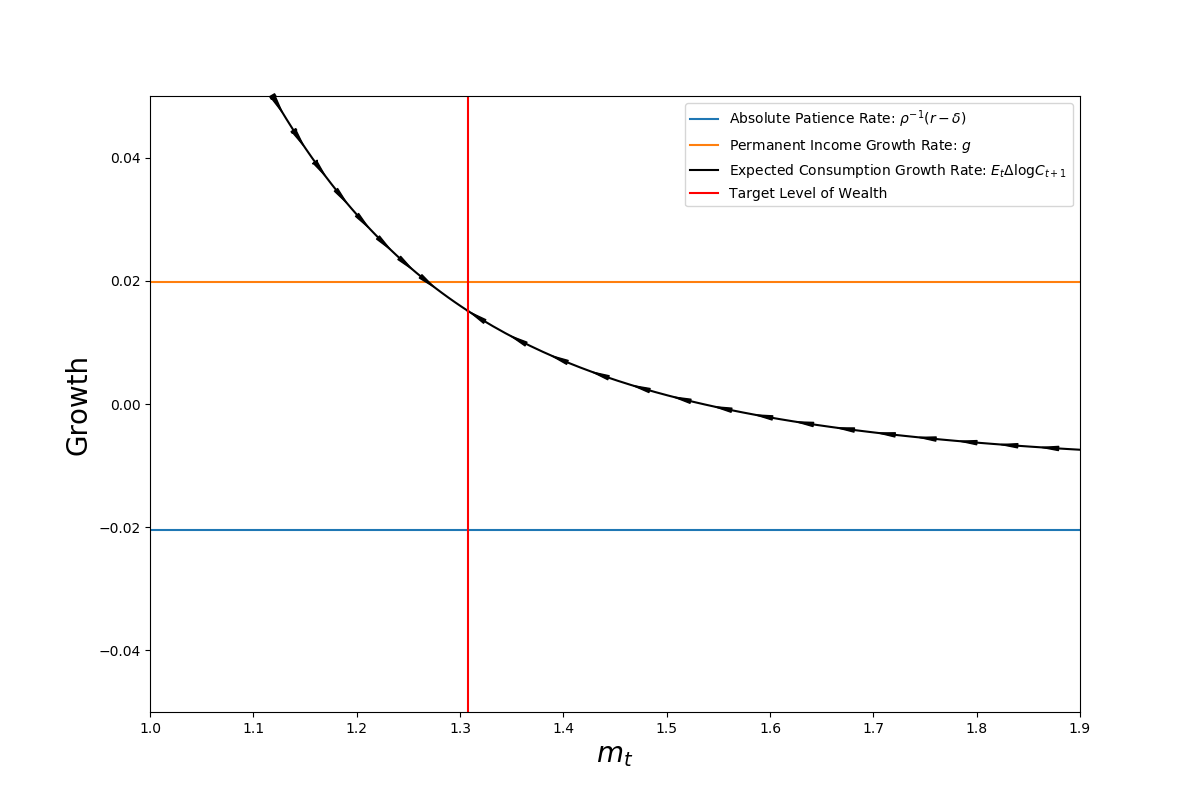
\includegraphics[width=6in]{Figures/Figure1a.png}}
\label{figure:1}
\caption{Expected Consumption Growth as a Function of Cash on Hand}
\end{figure}
\end{center}


\newpage

\section{Appendix}

%\begin{tabular}{lrrrrrrr}
\toprule
{} &  Growth rate of aggregate consumption &  Average growth rate of household permanent income &  Average growth rate of household consumption &  Aggregate personal saving rate &  Average MPC out of wealth &  Average net wealth &  Target net wealth \\
\midrule
Base Value         &                              0.020957 &                                           0.014807 &                                      0.014978 &                        0.006265 &                   0.315820 &            0.341770 &           0.313770 \\
g = .04            &                              0.040290 &                                           0.034225 &                                      0.034508 &                        0.009891 &                   0.414938 &            0.265945 &           0.246728 \\
depreciation = .10 &                              0.020821 &                                           0.014807 &                                      0.015143 &                        0.004310 &                   0.477366 &            0.230806 &           0.214614 \\
\bottomrule
\end{tabular}


\begin{table}[H]
	\label{table:1}
	\centerline{\scalebox{.5}{\begin{tabular}{lrrrrrrr}
\toprule
{} &  Growth rate of aggregate consumption &  Average growth rate of household permanent income &  Average growth rate of household consumption &  Aggregate personal saving rate &  Average MPC out of wealth &  Average net wealth &  Target net wealth \\
\midrule
Base Value         &                              0.020957 &                                           0.014807 &                                      0.014978 &                        0.006265 &                   0.315820 &            0.341770 &           0.313770 \\
g = .04            &                              0.040290 &                                           0.034225 &                                      0.034508 &                        0.009891 &                   0.414938 &            0.265945 &           0.246728 \\
depreciation = .10 &                              0.020821 &                                           0.014807 &                                      0.015143 &                        0.004310 &                   0.477366 &            0.230806 &           0.214614 \\
\bottomrule
\end{tabular}
}}
\end{table}

\newpage

\nocite{*}
\bibliographystyle{apacite}
\bibliography{\RefDir/Carroll1997}


\end{document}